\documentclass{beamer}
\usetheme{Boadilla}
\usepackage{hyperref}
\usepackage[T1]{fontenc}

% other packages
\usepackage{latexsym,amsmath,xcolor,multicol,booktabs,calligra}
\usepackage{graphicx,pstricks,listings,stackengine}
\usepackage{amsfonts}
\usepackage{enumerate}
\usepackage{amsmath}
\usepackage{amssymb}
\usepackage{amsthm}
\usepackage{url}
\usepackage[spanish]{babel}
\usepackage{enumitem}
\setbeamercovered{transparent}


\title{Software Libre Para Una Sociedad Libre}
\author{GNUTADEO}
\institute{UTADEO}
\date{18 de julio}

\begin{document}

\begin{frame}
  \titlepage
\end{frame}

\begin{frame}
 \frametitle{Índice} \tableofcontents[sectionstyle=show,subsectionstyle=show/shaded/hide,subsubsectionstyle=show/shaded/hide,currentsection]
\end{frame}

\AtBeginSection[]
{
  \begin{frame}
    \tableofcontents[sectionstyle=show/shaded,subsectionstyle=show/shaded/hide,subsubsectionstyle=show/shaded/hide]
  \end{frame}
}

\section{¿Qué es el Movimiento del Software Libre?}
\AtBeginSubsection[]
{
  \begin{frame}
    \tableofcontents[sectionstyle=show/shaded,subsectionstyle=show/shaded/hide,subsubsectionstyle=show/shaded/hide]
  \end{frame}
}
\subsection{Origenes}

\AtBeginSubsubsection[]
{
  \begin{frame}
    \tableofcontents[sectionstyle=show/shaded,subsectionstyle=show/shaded/hide,subsubsectionstyle=show/shaded/hide]
  \end{frame}
}
\subsubsection{Antes de GNU}

\begin{frame}
  \frametitle{La computación antes de los 80's}
  \begin{columns}
    \column{0.4\textwidth}
    \begin{itemize}
      \item Todo software era hecho por académicos trabajando en colaboración.
    \end{itemize}

    \column{0.6\textwidth}
    \begin{figure}[H]
      \centering
      
\includegraphics[width=\linewidth]{img/Image1.jpg}
    \end{figure}
  \end{columns}
\end{frame}


\AtBeginSubsubsection[]
{
  \begin{frame}
    \tableofcontents[sectionstyle=show/shaded,subsectionstyle=show/shaded/hide,subsubsectionstyle=show/shaded/hide]
  \end{frame}
}
\subsubsection{Richard Stallman}

\begin{frame}
  \frametitle{MIT--1980}
  \begin{figure}[H]
    \centering
    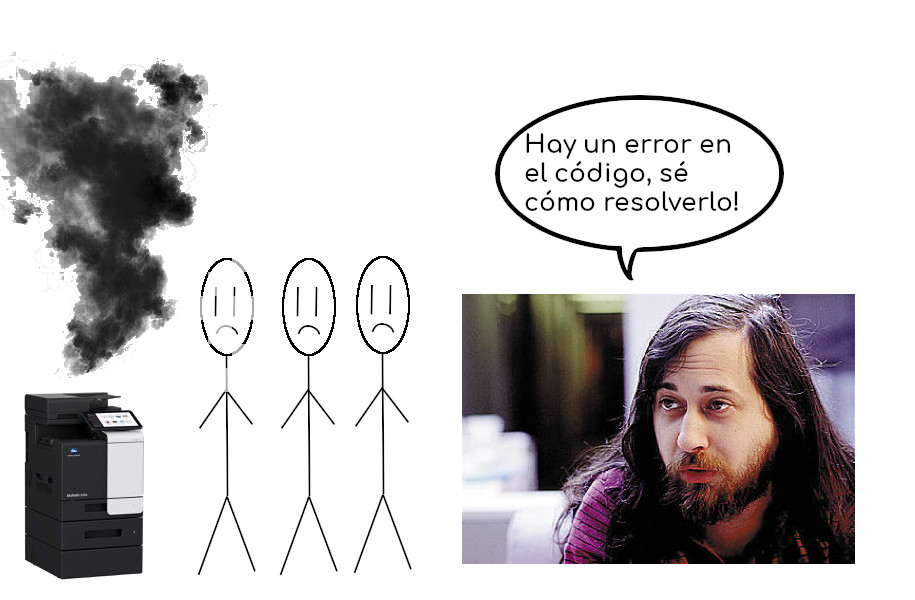
\includegraphics[width=\linewidth]{img/Image2.jpg}
  \end{figure}
\end{frame}

\begin{frame}
  \begin{figure}[H]
    \centering
    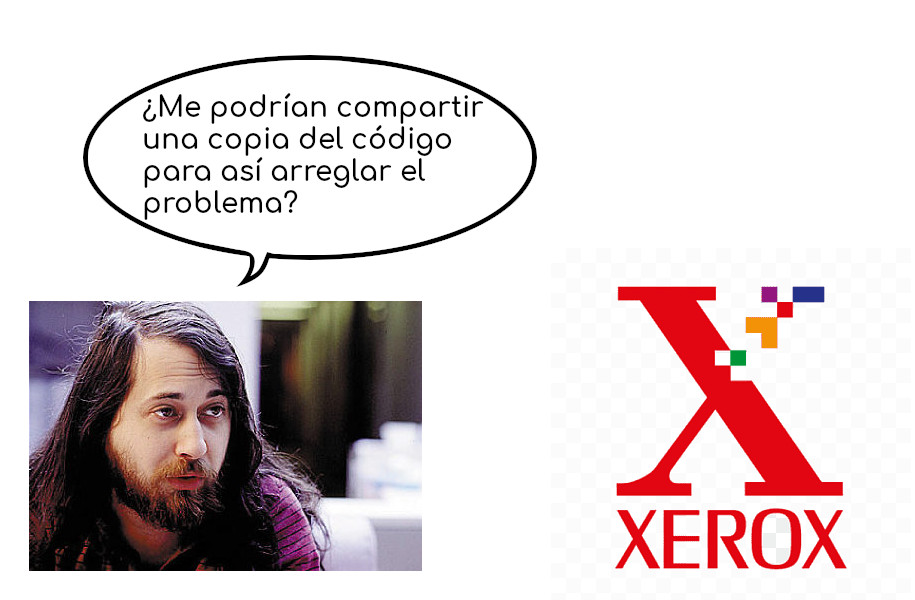
\includegraphics[width=\linewidth]{img/Image3.jpg}
  \end{figure}
\end{frame}

\begin{frame}
  \begin{figure}[H]
    \centering
    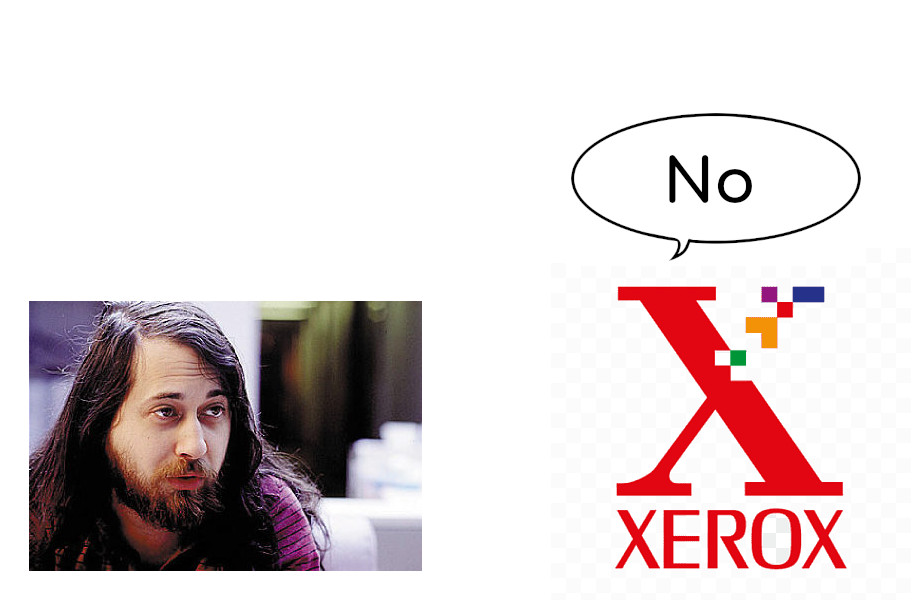
\includegraphics[width=\linewidth]{img/Image4.jpg}
  \end{figure}
\end{frame}

\begin{frame}
  \begin{figure}[H]
    \centering
    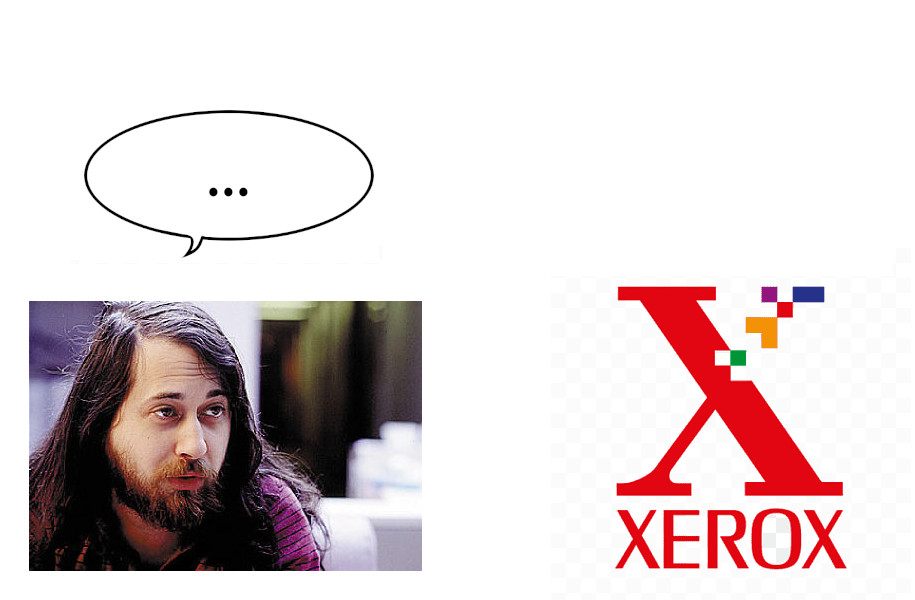
\includegraphics[width=\linewidth]{img/Image5.jpg}
  \end{figure}
\end{frame}


\AtBeginSubsubsection[]
{
  \begin{frame}
    \tableofcontents[sectionstyle=show/shaded,subsectionstyle=show/shaded/hide,subsubsectionstyle=show/shaded/hide]
  \end{frame}
}
\subsubsection{UNIX}
\begin{frame}
  \frametitle{UNIX}
  \begin{columns}
    \column{0.4\textwidth}
    \begin{itemize}
      \item Filosofía UNIX.
      \item ``La potencia de un sistema viene de las relaciones entre los programas mas que los programas por sí solos.''
    \end{itemize}

    \column{0.6\textwidth}
    \begin{figure}[H]
      \centering
      
\includegraphics[width=\linewidth]{img/UNIX.png}
    \end{figure}
  \end{columns}
\end{frame}

\AtBeginSubsubsection[]
{
  \begin{frame}
    \tableofcontents[sectionstyle=show/shaded,subsectionstyle=show/shaded/hide,subsubsectionstyle=show/shaded/hide]
  \end{frame}
}
\subsubsection{GNU}
\begin{frame}
  \frametitle{GNU's Not Unix}
  \begin{figure}[H]
    \centering
    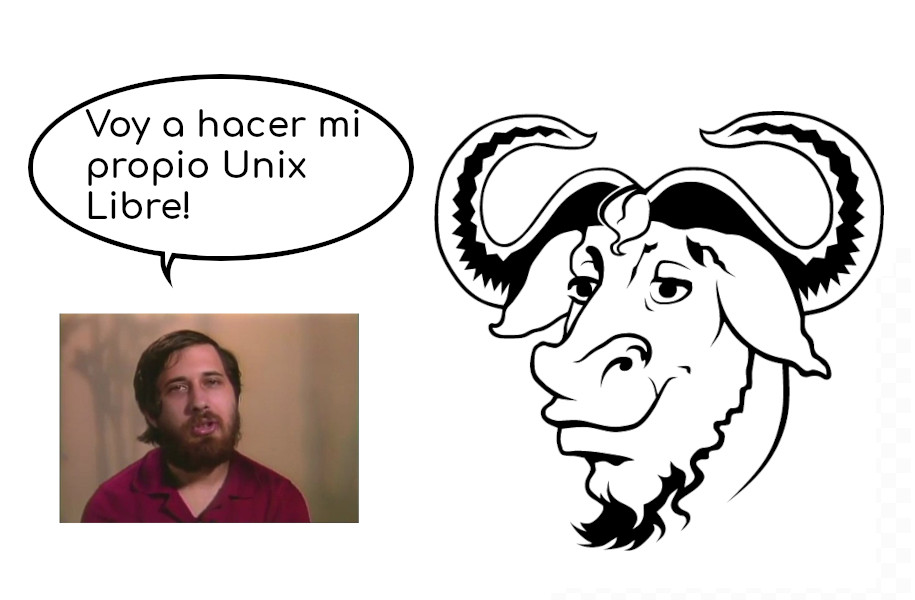
\includegraphics[width=\textwidth]{img/Image6.jpg}
  \end{figure}
\end{frame}

\begin{frame}
  \begin{figure}[H]
    \centering
    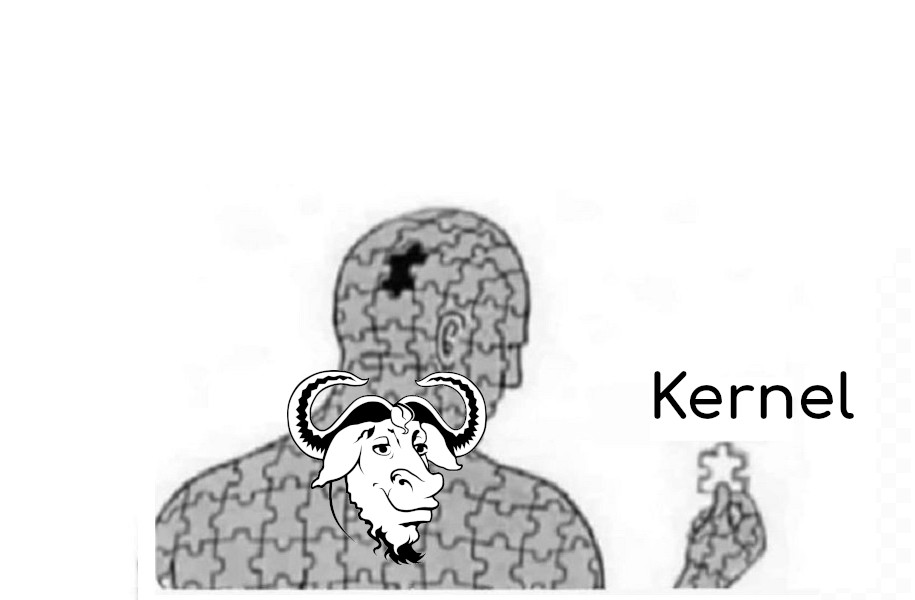
\includegraphics[width=\textwidth]{img/Image7.jpg}
  \end{figure}
\end{frame}


\AtBeginSubsubsection[]
{
  \begin{frame}
    \tableofcontents[sectionstyle=show/shaded,subsectionstyle=show/shaded/hide,subsubsectionstyle=show/shaded/hide]
  \end{frame}
}
\subsubsection{Linux}
\begin{frame}
  \frametitle{Linus Torvalds-Finlandia, 1992}
  \begin{figure}[H]
    \centering
    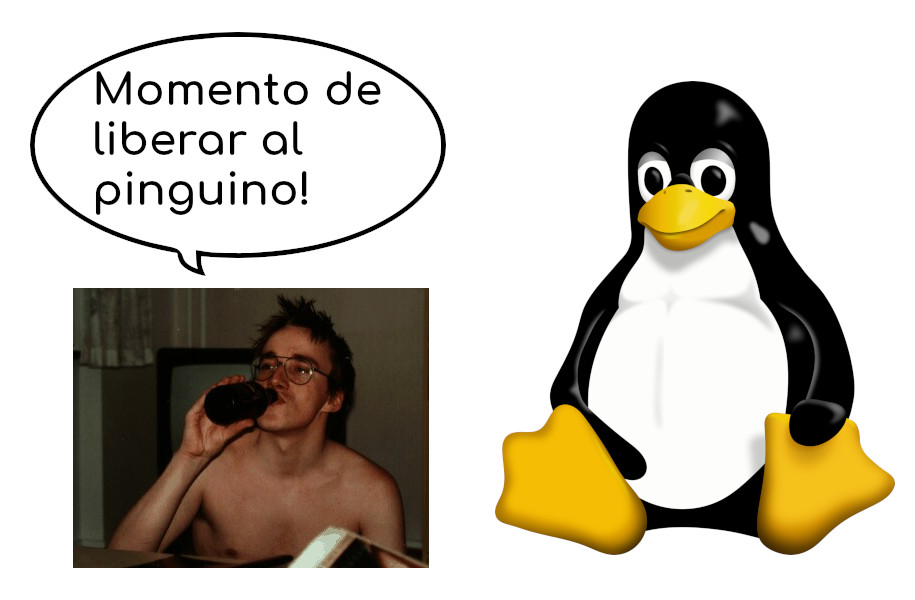
\includegraphics[width=\textwidth]{img/Image8.jpg}
  \end{figure}
\end{frame}

 \begin{frame}
  \frametitle{GNU + Linux}
  \begin{figure}[H]
    \centering
    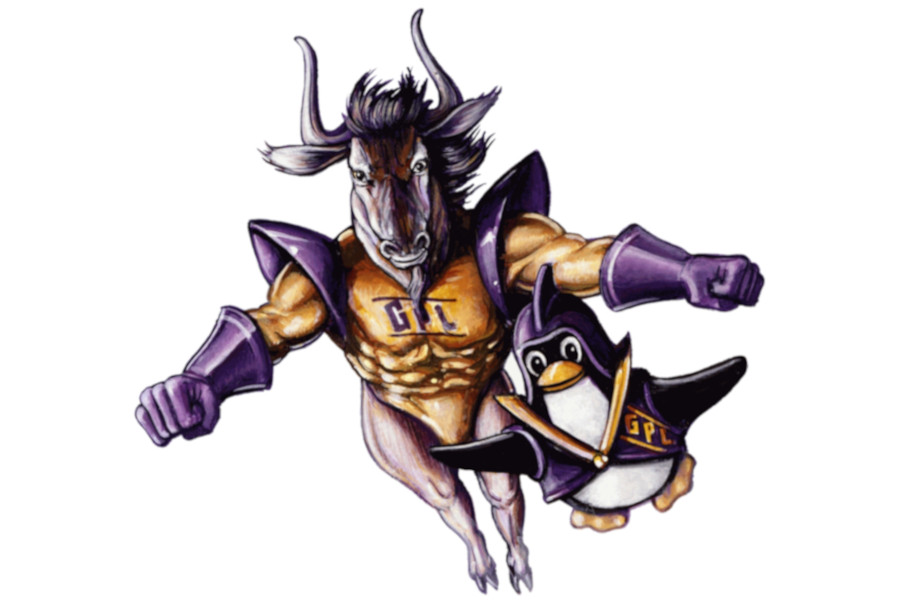
\includegraphics[width=\textwidth]{img/Image9.jpg}
  \end{figure}
\end{frame}

\begin{frame}
  \frametitle{Los 4 mandamientos (o libertades) del Software Libre}
  \begin{columns}
    \column{0.5\textwidth}
    \begin{figure}[H]
      \centering
      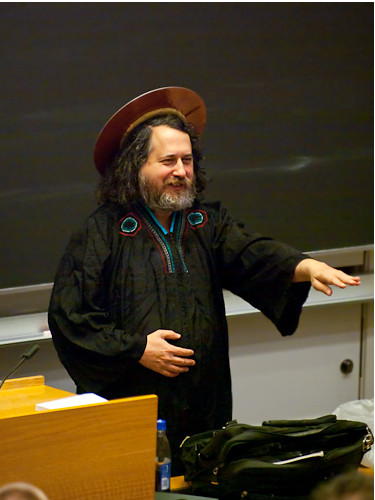
\includegraphics[width=0.8\textwidth]{img/Image10.jpg}
      \caption{San Ignucius (Richard Stallman)}
    \end{figure}

    \column{0.5\textwidth}
    \begin{enumerate}[start=0]
      \item \textbf{Usar} el programa como desees.
      \item \textbf{Estudiar} cómo funciona el programa, y cambiarlo para hacer lo que desees.
      \item \textbf{Redistribuir} y hacer \textbf{copias} para ayudar al prójimo.
      \item \textbf{Mejorar} el programa, y publicar tus mejoras para que toda la comunidad se beneficie.
    \end{enumerate}
  \end{columns}
\end{frame}

\AtBeginSection[]
{
  \begin{frame}
    \tableofcontents[sectionstyle=show/shaded,subsectionstyle=show/shaded/hide,sectionstyle=show/shaded/hide]
  \end{frame}
}
\section{Software Libre, propietario y grátis}


\AtBeginSubsection[]
{
  \begin{frame}
    \tableofcontents[sectionstyle=show/shaded,subsectionstyle=show/shaded/hide,subsectionstyle=show/shaded/hide]
  \end{frame}
}

\subsection{Software Libre}


\begin{frame}
  \frametitle{Software Libre}
  \centering
  \begin{figure}[H]
    \centering
    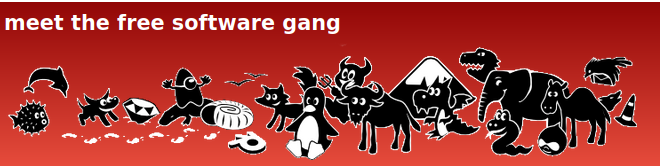
\includegraphics[width=\textwidth]{img/Image11.png}
  \end{figure}
\end{frame}

\AtBeginSubsection[]
{
  \begin{frame}
    \tableofcontents[sectionstyle=show/shaded,subsectionstyle=show/shaded/hide,subsectionstyle=show/shaded/hide]
  \end{frame}
}

\subsection{Software Propietario}


\begin{frame}
  \frametitle{Software Propietario}
  \centering
  \begin{columns}
    \column{0.5\textwidth}
    \begin{figure}[H]
      \centering
      
\includegraphics[width=1\textwidth]{img/Image12.jpg}
    \end{figure}

    \column{0.5\textwidth}
    \begin{itemize}
      \item No respeta la libertad del usuario.
      \item Sus licencias son abusivas.
      \item Piensan exclusivamente en el beneficio monetario en lugar del bien de la sociedad.
    \end{itemize}
  \end{columns}
\end{frame}


\AtBeginSubsection[]
{
  \begin{frame}
    \tableofcontents[sectionstyle=show/shaded,subsectionstyle=show/shaded/hide,subsectionstyle=show/shaded/hide]
  \end{frame}
}

\subsection{Software Grátis}

\begin{frame}
  \frametitle{Software Grátis}
  \centering
  \begin{columns}
    \column{0.5\textwidth}
    \begin{figure}[H]
      \centering
      
\includegraphics[width=\textwidth]{img/Image13.jpg}
    \end{figure}

    \column{0.5\textwidth}
    \begin{itemize}
      \item No impone ninguna barrera para su adquisición.
      \item No respeta la información y los datos de los usuarios.
      \item No comparten acceso al código fuente.
    \end{itemize}
  \end{columns}
\end{frame}

\AtBeginSection[]
{
  \begin{frame}
    \tableofcontents[sectionstyle=show/shaded,subsectionstyle=show/shaded/hide,subsubsectionstyle=show/shaded/hide]
  \end{frame}
}
\section{Importancia del Software Libre en la sociedad actual}
\begin{frame}
  \centering
  \frametitle{Uso de Sistemas Operativos en computadores de Escritorio}
  \begin{figure}[H]
    \centering
    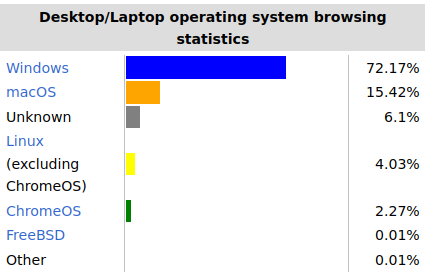
\includegraphics[width=0.8\textwidth]{img/StatsDesktop.png}
  \end{figure}
\end{frame}

\begin{frame}
  \centering
  \frametitle{Usos de Sistemas Operativos en Servidores}
  \begin{table}
    \begin{tabular}{|c|c|c|c|}
      \hline
      \textbf{Fuente} & \textbf{Fecha} & \textbf{Unix, Linux} & \textbf{Microsoft Windows} \\ \hline
      W3Techs & 14 de julio 2022 & 80.1\% & 20.1\% \\ \hline
      Seguridad & Febrero de 2014 & \(<79.3\%\) & \(>20.7\%\) \\ \hline
    \end{tabular}
  \end{table}
\end{frame}

\begin{frame}
  \centering
  \frametitle{Usos de Sistemas Operativos en Super computadoras}
  \begin{figure}[H]
    \centering
    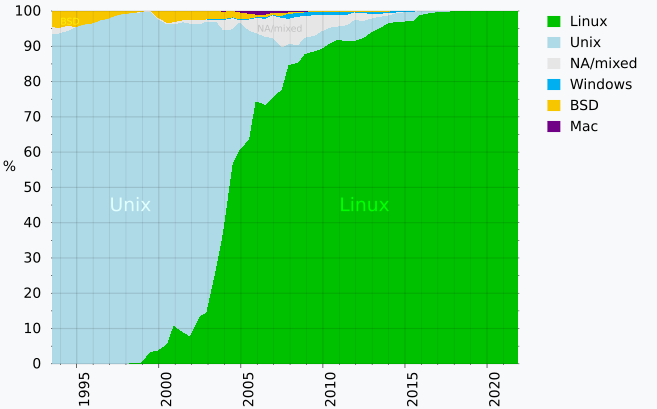
\includegraphics[width=0.8\textwidth]{img/StatsSPC.png}
  \end{figure}
\end{frame}

\begin{frame}
  \centering
  \frametitle{Uso en la vida cotidiana...}
  \begin{figure}[H]
    \centering
    
\includegraphics[width=0.8\textwidth]{img/Image14.jpg}
  \end{figure}
\end{frame}


\AtBeginSection[]
{
  \begin{frame}
    \tableofcontents[sectionstyle=show/shaded,subsectionstyle=show/shaded/hide,subsubsectionstyle=show/shaded/hide]
  \end{frame}
}
\section{¿Cómo podemos colaborar?}

\begin{frame}
  \frametitle{Formando comunidades y compartiendo con otras personas!}
  \begin{columns}
    \centering
    \column{0.5\textwidth}
    \begin{itemize}
      \item Empezando a utilizar alternativas libres y abiertas en tú día a día.
      \item Divulgando la filosofía del Software Libre.
      \item Haciendo aportaciones a proyectos libres.
    \end{itemize}

    \column{0.5\textwidth}
    \begin{figure}[H]
      \centering
      
\includegraphics[width=\textwidth]{img/LogoGNUTADEO.jpg}
    \end{figure}
  \end{columns}
\end{frame}

\begin{frame}
  \centering
  \frametitle{Nuestro trabajo como colectivo}
  \begin{figure}[H]
    \centering
    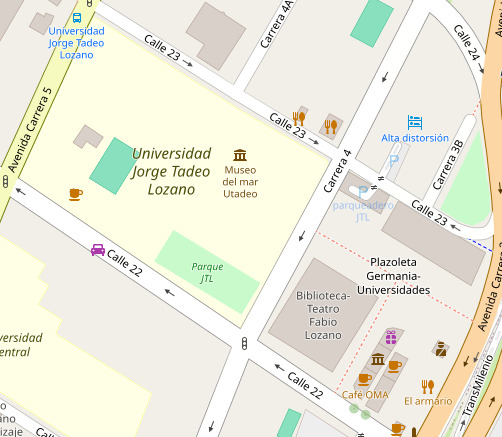
\includegraphics[width=0.6\textwidth]{img/UtadeoAntes.jpg}
    \caption{Mapa de Utadeo en OpenStreetMap, fecha 18 de junio 2024}
  \end{figure}
\end{frame}

\begin{frame}
  \centering
  \frametitle{Nuestro avance en la universidad}
  \begin{figure}[H]
    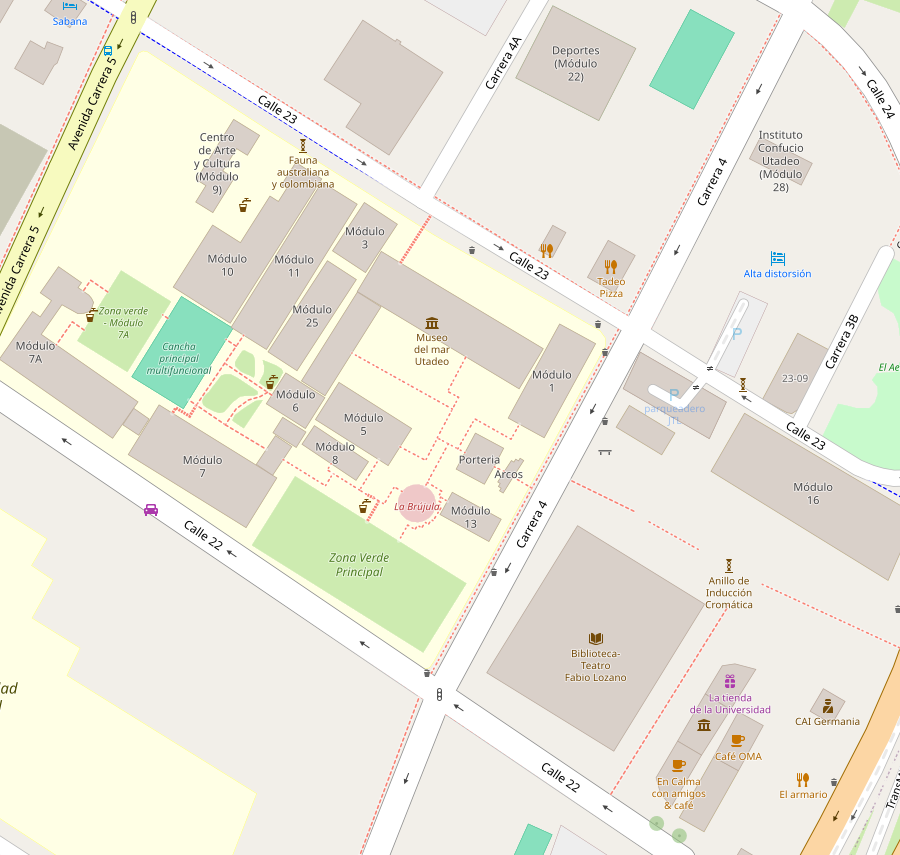
\includegraphics[width=0.7\textwidth]{img/UtadeoAhora.png}
  \end{figure}
\end{frame}



\begin{frame}
  \begin{columns}
    \centering
    \column{0.5\textwidth}
    \begin{figure}[H]
      \centering
      \includegraphics[scale=0.15]{~/todo-mio/UTADEO/COLECTIVO/Enlaces WP e IG/Instagram.jpeg}
    \end{figure}

    \column{0.5\textwidth}
    \begin{figure}[H]
      \centering
      \includegraphics[scale=0.15]{~/todo-mio/UTADEO/COLECTIVO/Enlaces WP e IG/Formulario.jpg}
    \end{figure}
  \end{columns}
\end{frame}


\begin{frame}
  \centering
  \frametitle{Presentación hecha únicamente con Software Libre}
  \begin{figure}[H]
    \centering
    
\includegraphics[scale=1.2]{img/SoftwareUsado.png}
  \end{figure}
\end{frame}


\end{document}
